\chapter{Foundation}

Structure of PASS descriptions and ts relation to the execution semantics defined as Abstract State Machines (ASM).

\begin{itemize}
	\item Start Event
	\item Intermediate Event
	\item End Event
\end{itemize}

Structure of each chapter docuement

\begin{itemize}
	\item Informal description of PASS aspects
	\item OWL Description of these aspects
	\item ASM Sematic
\end{itemize}

In order to facilitate the understanding of the following sections we will introduce the philosophy of subject-orienting modelling which is the underlying Parallel Activity Specification Scheme (PASS). Additional we will give a short introduction to ontologies, especially the Web Ontology Language (OWL), and to Abstract State Machines (ASM) as underlying concepts of this standard document.

\section{Subject Orientation and PASS }
\label{SubjectOrient}

\sidepar{Text in the sidebar}

In this section we lay ground for PASS as a language for describing proceses in a subjectoriented way. This section is not a complete description of all PASS features it only gives a first impression about subject orientation and the specification language PASS. The advanced features are defined in the ubpcoming chapters.

The term subject has manifold meanings depending on the discipline. In philosophy a subject is an observer and an object is a thing observed. In the grammar of many languages the term subject has a slightly different meaning. “According to the traditional view, subject is the doer of the action (actor) or the element that expresses what the sentence is about (topic).”(see E. L. Keenan; Towards a universal definition of 'subject'. Subject and topic, ed. by  Charles N. Li,: Academic Press New York 1976 ). In PASS the term subject coreponds to the doer of an action whereas in ontology description languages like RDF (see section \ref{IntroOntology} ) the term subject means the topic what the "sentence" is about.

\subsection{Subject-driven Business Processes}

Subjects represent the behavior of an active entity. A specification of a subject does not say anything about the technology used to execute the described behavior. This is different to other encapsulation approaches, such as multi-agent systems.

Subjects communicate with each other by exchanging messages. Messages have a name and a payload. The name should express the meaning of a message informally and the payloads are the data (business objects) transported. Internally, subjects execute local activities such as calculating a price, storing an address etc.

A subject sends messages to other subjects, expects messages from other subjects, and executes internal actions. All these activities are done in sequences which are defined in a subject's behavior specification.
Subject-oriented process specifications are embedded in a context. A context is defined by the business organization and the technology by which a business process is executed.

Subject-oriented system development integrates established theories and concepts. It has been inspired by various process algebras (see e.g. [2], [3], [4]), by the basic structure of nearly all natural languages (Subject, Predicate, Object) and the systemic sociology developed by Niklas Luhmann (an introduction can be found in [5]). According to the organizational theory developed by Luhmann the smallest organization consists of communication executed between at least two information processing entities [5]. The integrated concepts have been enhanced and adapted to organizational stakeholder requirements, such as providing a simple graphical notation, as detailed in the following sections.

\subsection{Subject Interaction and Behavior}

We introduce the basic concepts of process modeling in S-BPM using a simple order process. A customer sends an order to the order handling department of a supplier. He is going to receive an order confirmation and the ordered product by the shipment company. Figure \ref{fig:ordercomstructure} shows the communication structure of that process. The involved subjects and the messages they exchange can easily be grasped. 

\strictpagecheck
\begin{figure}[htbp]
	\begin{sidecaption}[The Communication Structure in the Order Process]{The Communication Structure in the Order Process}
	\centering
	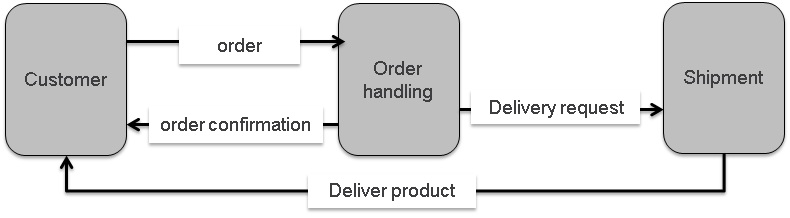
\includegraphics[width=0.7\linewidth]{20181026-Ontologie-Bilder/Grafiken-Ontologie/SUbjectExecution/OrderComStructure}
	\end{sidecaption}
	\label{fig:ordercomstructure}
\end{figure}

Each subject has a so-called input pool which is its mail box for receiving messages. This input pool can be structured according to the business requirements at hand. The modeler can define how many messages of which type and/or from which sender can be deposited and what the reaction is if these restrictions are violated. This means the synchronization through message exchange can be specified for each subject individually.
Messages have an intuitive meaning expressed by their name. A formal semantic is given by their use and the data which are transported with a message. Figure \ref{fig:ordercustomerorderhandling} depicts the behavior of the subjects "customer" and "order handling".

\strictpagecheck
\begin{figure}[htbp]
	\begin{sidecaption}[The Behavior of Subjects]{The Behavior of Subjects}
	\centering
	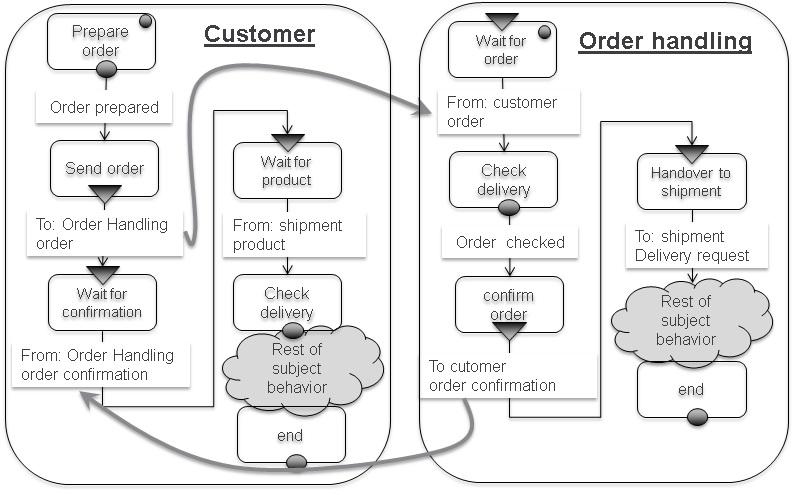
\includegraphics[width=0.9\linewidth]{20181026-Ontologie-Bilder/Grafiken-Ontologie/SUbjectExecution/OrderCustomerOrderHandling}
	\end{sidecaption}
	\label{fig:ordercustomerorderhandling}
\end{figure}

In the first state of its behavior the subject "customer" executes the internal function "Prepare order". When this function is finished the transition "order prepared" follows. In the succeeding state "send order" the message "order" is sent to the subject "order handling". After this message is sent (deposited in the input pool of subject "order handling"), the subject "Customer" goes into the state "wait for confirmation". If this message is not in the input pool the subject stops its execution, until the corresponding message arrives in the input pool. On arrival the subject removes the message from the input pool and follows the transition into state "Wait for product" and so on.

The subject "Order Handling" waits for the message "order" from the subject "customer". If this message is in the input pool it is removed and the succeeding function "check order" is executed and so on.

The behavior of each subject describes in which order it sends messages, expects (receives) and performs internal functions. Messages transport data from the sending to the receiving subject, and internal functions operate on internal data of a subject. These data aspects of a subject are described in section \ref{SUbjects-Objects} In a dynamic and fast changing world, processes need to  be able to capture known but unpredictable events. In our example let us assume that a customer can change an order. This means the subject "customer" may send the message "Change order" at any time. Figure \ref{fig:ordercomstructure} shows the corresponding communication structure, which now contains the message "change order".

\strictpagecheck
\begin{figure}[htbp]
	\begin{sidecaption}[The Communication Structure with Change Message]{The Communication Structure with Change Message}
	\centering
	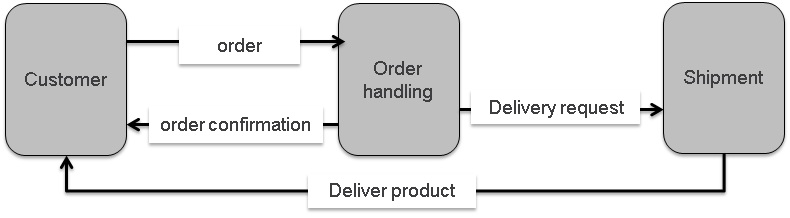
\includegraphics[width=0.7\linewidth]{20181026-Ontologie-Bilder/Grafiken-Ontologie/SUbjectExecution/OrderComStructure}
	\end{sidecaption}
	\label{fig:ordercomstructure}
\end{figure}

Due to this unpredictable event the behavior of the involved subjects needs also to be adapted. Figure \ref{fig:ordercustomerchange} illustrates the respective behavior of the customer. 

\strictpagecheck
\begin{figure}[ph]
	\centering
	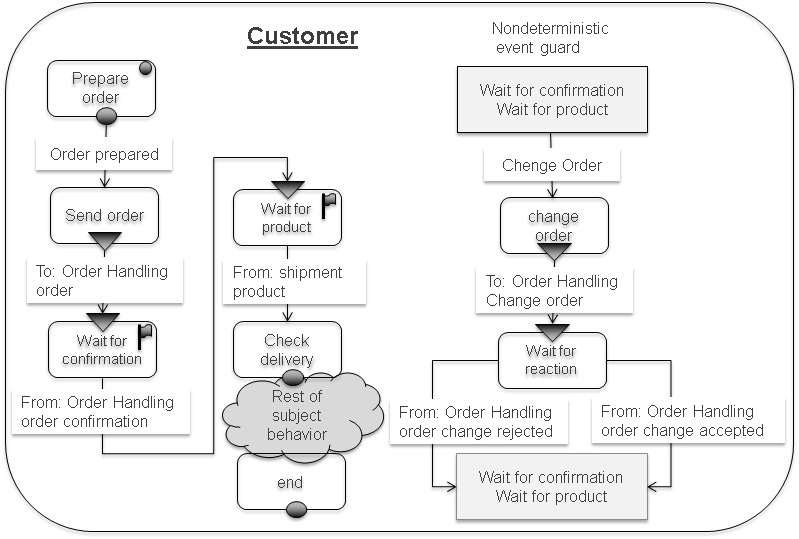
\includegraphics[width=0.7\linewidth]{20181026-Ontologie-Bilder/Grafiken-Ontologie/SUbjectExecution/OrderCustomerChange}
	\caption[Customer is allowed to Change Orders]{Customer is allowed to Change Orders}
	\label{fig:ordercustomerchange}
\end{figure}


The subject "customer" may have the idea to change its order in the state "wait for confirmation" or in the state "wait for product". The flags in these states indicate that there is a so-called behavior extension described by a so-called nondeterministic event guard [12, 22]. The non-deterministic event created in the subject is the idea "change order". If this idea comes up, the current states, either "wait for confirmation" or "wait for product", are left, and the subject "customer" jumps into state "change order" in the guard behavior. In this state the message "change order" is sent and the subject waits in state "wait for reaction". In this state the answer can either be "order change accepted" or "order change rejected". Independently of the received message the subject "customer" moves to the state "wait for product". The message "order change accepted" is considered as confirmation, if a confirmation has not arrived yet (state "wait for confirmation"). If the change is rejected the customer has to wait for the product(s) he/she has ordered originally.
Similar to the behavior of the subject "customer" the behavior of the subject "order handling" has to be adapted.


\subsection{Subjects and Objects}
\label{SUbjects-Objects}

Up to now we did not mention data or the objects with their predicates, in order to get complete sentences comprising subject, predicate, and object. Figure \ref{fig:subjectobject} displays how subjects and objects are connected. The internal function "prepare order" uses internal data to prepare the data for the order message. This order data is sent as payload of the message "order".

\begin{figure}[ph]
	\centering
	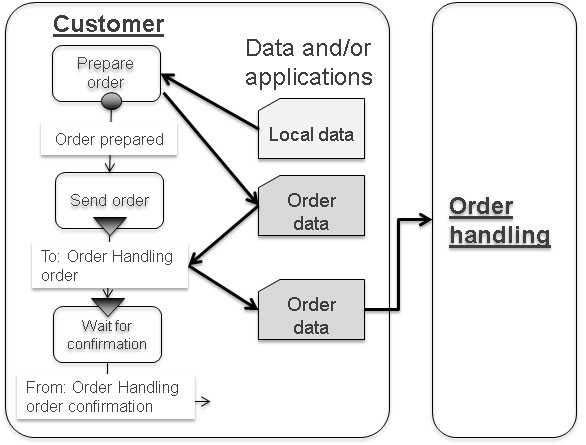
\includegraphics[width=0.7\linewidth]{20181026-Ontologie-Bilder/Grafiken-Ontologie/SUbjectExecution/SUbjectObject}
	\caption[Subjects and Objects]{Subjects and Objects}
	\label{fig:subjectobject}
\end{figure}

The internal functions in a subject can be realized as methods of an object or functions implemented in a service, if a service-oriented architecture is available. These objects have an additional method for each message. If a message is sent, the method allows receiving data values sent with the message, and if a message is received the corresponding method is used to store the received data in the object [22]. This means either subjects are the entities which use synchronous services as implementation of functions or asynchronous services are implemented through subjects or even through complex processes consisting of several subjects. Consequently, , the concept Service Oriented Architecture (SOA) is complementary to S-BPM: Subjects are the entities which use the services offered by SOAs (cf. [25]).

\section{Introduction to Ontologies and OWL }
\label{IntroOntology}

This short introduction to ontology, the Resource Description Framework and Web Ontology Language (OWL) should help to get an understanding of the PASS ontology outlined in section \ref{PASSStruct} and \ref{PASSExec}.\\
Ontologies are a formal way to describe taxonomies and classification networks, essentially defining the structure of knowledge for various domains: the nouns representing classes of objects and the verbs representing relations between the objects of classes.\\
In computer science and information science, an ontology encompasses a representation, formal naming, and definition of the classes, properties, and relations between the data, and entities that substantiate considered domains.\\

The Resource Description Framework (RDF) provides a graph-based data model or framework for structuring data as statements about resources. A “resource” may be any “thing” that exists in the world: a person, place, event, book, museum object, but also an abstract concept like data objects.
The following figure \ref{fig:classes-properties}  shows an RDF graph.

\strictpagecheck
\begin{figure}[h]
	\centering
	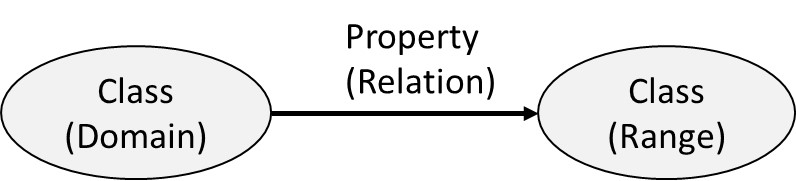
\includegraphics[width=0.6\linewidth]{20181026-Ontologie-Bilder/Grafiken-Ontologie/Introduction/Classes-Properties}
	\begin{sidecaption}
		[RDF graphic]{RDF graphic}
	\end{sidecaption}
	\label{fig:classes-properties}
\end{figure}

RDF is based on the idea of making statements about resources (in particular web resources) in expressions of the form subject–predicate–object, known as triples. The subject denotes the resource, and the predicate denotes traits or aspects of the resource, and expresses a relationship between the subject and the object. In the context of ontology the term subject expresses what the sentence is about (topic) (see \ref{SubjectOrient}).

For describing ontologies several languages have been developed. One widely used langauge is OWL (world wide web ontology language) which is based on the Resource Description Framework (RDF).

OWL has classes, properties and instances. Classes represents terms also called concepts. Classes have properties and instances are individuals of one or more classes.

A class is a type of thing. A type of “resource” in the RDF sense can be
person, place, object, concept, event, etc.. Classes and subclasses form a hierarchical taxonomy and members of a subclass inherit the characteristics of their parent class (superclass). Everything whichis true for the parent class is also true for the subclass.

A member of a subclass “is a”, or “is a kind of” its parent class.\\
Ontologies define a set of properties used in a specific knowledge domain. In an ontology context, properties relate members of one class to members of another class, or to a literal.

Domains and ranges define restrictions on properties. A domain restricts what kinds of resources or members of a class can be the subject of a given property in an RDF triple.A range restricts what kinds of resources / members of a
class or data types (literals) can be the object of a given property in an RDF triple.

Entities belonging to a certain class are instances of this class or inviduals. A simple ontology with various classes, properties and individual is shown below:

Ontology statement examples:
\begin{itemize}
	\item \textbf {Class definition statements:}
	\begin{itemize}
		\item Parent isA Class
		\item Mother isA Class
		\item Mother subClassOf Parent
		\item Child isA Class
	\end{itemize}
	\item \textbf {Property definition statement:}
	\begin{itemize}
		\item isMotherOf isA Property with domain Mother and range Child
	\end{itemize}
	\item \textbf{Individual/instance statements:}
	\begin{itemize}
		\item MariaSchmidt isA Mother
		\item MaxSchmidt isA Child
		\item MariaSchmidt isMotherOf MaxSchmidt
	\end{itemize}
\end{itemize}

\section{Introduction to Abstract State Machines }

An abstract state machine (ASM) is a state machine operating on states that are arbitrary data structures (structure in the sense of mathematical logic, that is a nonempty set together with a number of functions (operations) and relations over the set).

The language of the so called Abstract STate Machine uses only elementary If-Then-Else-rules which are typical also for rule systems formulated in natural language, i.e., rules of the (symbolic) form\
\textbf{if} \textit{Condition} \textbf{then} \textit{ACTION}\
with arbitrary \textit{Condition} and \textit{ACTION}. The latter is usually a finite set of assignments of form \textit{f (t1, ..., tn) := t}. The meaning of such a rule is to perform in any given state the indicated action if the indicated condition holds in this state.\ 

The unrestricted generality of the used notion of Condition and ACTION is guaranteed by using as ASM-states the so-called Tarski structures, i.e., arbitrary sets of arbitrary elements with arbitrary functions and relations defined on them. These structures are updatable by rules of the form above. In the case of business processes, the elements are placeholders for values of arbitrary type and the operations are typically the creation, duplication, deletion, or manipulation (value change) of objects. The so-called views are conceptually nothing else than projections (read: substructures) of such Tarski structures.\

An (asynchronous, also called distributed) ASM consists of a set of agents each of which is equipped with a set of rules of the above form, called its program. Every agent can execute in an arbitrary state in one step all its rules which are executable, i.e., whose condition is true in the indicated state. For this reason, such an ASM, if it has only one agent, is also called sequential ASM. In general, each agent has its own ‘time’ to execute a step, in particular if its step is independent of the steps of other agents;  in special cases multiple agents can also execute their steps simultaneously (in a synchronous manner).\

Without further explanations, we adopt usual notations, abbreviations, etc., for example:\\
\textbf{if} \textit{Cond} \textbf{then} \textit{M1} else \textit{M2}\\
instead of the equivalent ASM with two rules:\\
\textbf{if} \textit{Cond} \textbf{then} \textit{M1} \\
\textbf{if} \textbf{not} \textit{Cond} \textbf{then} \textit{M2}\\
Another notation used below is\\
\textbf{let} \textit{x = t} \textbf{in} \textit{M}\\
for M(x/a), where a denotes the value of t in the given state and M(x/a) is obtained from M by substitution of each (free) occurrence of x in M by a.

For details of a mathematical definition of the semantics of ASMs which justifies their intuitive (rule-based or pseudo-code) understanding, we refer the reader to the AsmBook Börger, E., Stärk R. Abstract State Machines. A Method for High-Level System Design and Analysis. Springer, 2003.






